The assignment of this report conveyed critizing and accessing system-level Internet of Things components in scientififc literature.
Because the assigned paper \cite{paper} did not include anything IoT related, we will present our own idea.
In this section we will provide a short introduction to the Internet of Things and its key features, we will also present our idea and focus on the practicality and entrpreneurial aspect of the idea.

The Internet of Things refers to uniquely identitfiable objects, or things, and their virtual representations in an Internet-like structure. \cite{lecture}.
The intelligent application is the key feature here.
Important aspects to be taken into consideration when designing such systems are security, privacy and scalability.

The anatomy of Internet of Things is initiated by a certain event, that is detected and logged by devices that include self-properties \cite{lecture}.
This data is then uploaded by a ubiquitous and interoperable network.
The unique feature of the internet of things is that this system is smart and can generate knowledge and by analyzing this data and understands the system.
Certain events are then triggered and reported as response.
The intelligence of these systems lie in the adapting mechanisms that analyse and understand the environment in order to deal with the complex dynamics of a real-world environment.

Internet of Things has already been employed at multiple festivals and initially used as a ticketing solution in 2004 at the SXSW festival in Austin.
It emerged in the form of wristbands and cut down significantly on gate crashing and lost tickets \cite{thingmagic}.
SXSW announced that each tag contained a unique ID code, correlated with personal information availabe by SXSW \cite{sxsw}.
It has further been introduced at Coachella and Bonnaroo. \cite{coachella} \cite{bonnaroo}
RFID now even support cashlesh payments and integration with social networks, allowing people to upload pictures to facebook via the so-called "Live Click Stations"\cite{thingmagic}.
We can conlude that it safe to say that the Internet of Things hasn't reached its peak yet concerning festival and concerts.

Because our scenario already portrays users wearing a wristband throughout the festival containing the discussed electronics, we can add some small features to play into current trends concerning Internet of Things and music festivals.
By adding a RFID tag into each wristband, users are assigned unique IDs.
These tags can be applied fairly easy and can obviously contain functionality such as a unique entrance ID or even cashlesh payments.
In this report however, we want to focus on the fun factor of connecting with friends and strangers.
Users can prior to arriving at the festival use their unique ID and optionally link it to all the accounts of their friends are the accompanying social media.
When the users enter the festival site and receive their wristbands, these are connected to their unique id priorly received.
Whenever they charge their wristband, either at the bar or at check in points near every site of interest, their friends that are not near them will receive a message containing their location and if made, an image at the check-in location.
Based on certain check-in's at time in the schedule of the festival, the system can recognize their interests (if not already mentioned in their id page online) and even give them recommendations to go next to.
The sequence of this Internet of things can be seen in figure \ref{fig:iot}.

\begin{figure}[h!]
\centering
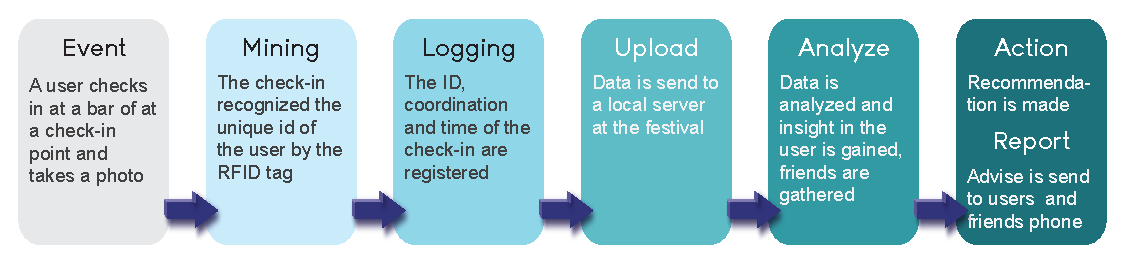
\includegraphics[width=1\textwidth]{IoT.pdf}
\caption{Internet of things chain of actions}
\label{fig:iot}
\end{figure}

Our system goed beyond simply assigning a unique id to a user, it also adds functionality and connects ids to exchange information. In this manner, it mines the data when users check in at charging points where they can even choose to make a picture.
These check-ins are logged and send to a server, where the users ID is processed and connected IDs of friends are notified.
The system can then analyze the data and generate knowledge by searching for common factors of interest.
Based on this intelligence, the system can in turn return some recommendations back to the user.
This doesn't just improve the experience of the user, but it gives the organization a better insight into the behavior of their visitors.









